\documentclass[11pt,twoside]{article}

\usepackage{asp2023}

\aspSuppressVolSlug
\resetcounters

\bibliographystyle{asp2021}

\markboth{Glorioso}{Cloud-Native Roman Science Processing}

\begin{document}

\title{Building a Cloud-Native, Petabyte-Scale Pipeline for the Roman Space Telescope}

\author{John Glorioso$^1$}
\affil{$^1$Space Telescope Science Institute, Baltimore, Maryland, United States; \email{jglorioso@stsci.edu}}

\paperauthor{John Glorioso}{jglorioso@stsci.edu}{}{Space Telescope Science Institute}{Data Management Division}{Baltimore}{Maryland}{21211}{United States}

%\aindex{Glorioso,~J.~G.}


\begin{abstract}
The Nancy Grace Roman Space Telescope is expected to produce at least 20 PB of data during its first five years, exceeding the practical processing capacity of existing on-premises mission infrastructure. The Space Telescope Science Institute (STScI) developed an event-driven system using Apache Airflow, Kubernetes, and AWS services to execute Roman science workflows with elastic cloud resources. We describe the architecture, its separation of orchestration from science computation, its worker model, and lessons from operation at scale.
\end{abstract}

\section{Mission Requirements}

STScI operates science data systems for the Hubble, James Webb, and Nancy Grace Roman space telescopes. Roman is expected to deliver approximately 1.375 TB per day \citep{GSFC13667}, more than 20 times Webb's volume and 500 times Hubble's. Data receipt and reprocessing campaigns produce workloads ranging from idle periods to thousands of simultaneous jobs.

The architecture must exchange data with mission partners, scale compute independently of orchestration, support concurrent software and reference-data versions, expose progress to operators, and return to minimal capacity when queues are empty.

These requirements led to an event-driven system in AWS in which object storage and queues form the durable boundaries between processing, archive ingest, and distribution.

\section{Event-Driven Processing Architecture}

Figure~\ref{fig:architecture} summarizes the end-to-end architecture. Raw data and delivery notifications originate in the Data Acquisition Processing and Handling Network Environment (DAPHNE), operated by NASA's Goddard Space Flight Center. Data products are stored as objects in Amazon Simple Storage Service (S3). Product-availability events are published through Amazon Simple Notification Service (SNS) and delivered to durable Amazon Simple Queue Service (SQS) queues.

\articlefigure[width=\textwidth]{C401_f1.eps} {fig:architecture} {Simplified Roman data flow.}

S3 is the authoritative object store, while notifications communicate work independently of data movement.

Apache Airflow expresses the processing dependencies as directed acyclic graphs. Lightweight tasks, including event handling, condition checking, and job coordination, execute through Airflow and its Celery workers. Memory and CPU intensive calibration tasks execute in separate Kubernetes pods on Amazon Elastic Kubernetes Service (EKS). This prevents long science jobs from occupying the limited scheduler and worker capacity needed to advance other workflows.

Science software is packaged as versioned container images in Amazon Elastic Container Registry (ECR). A workflow selects the required software and reference-data versions for a particular processing campaign. This supports controlled validation and reprocessing without replacing the software used by other campaigns. Infrastructure and deployment configuration are maintained as code, making the environments reproducible and allowing operating-system and container images to be updated without redeploying workflows.

Processing outputs are written to S3 and generate new availability events. Those events trigger higher processing levels. Archive records are written asynchronously in batches, avoiding individual database transactions for every product. Data is then made available through STScI archive services and to cloud-based analysis environments including the Roman Research Nexus.

\section{Elastic Execution}

EKS provides a common execution environment for Airflow services and science processing, but the two workload classes are isolated and scaled separately. Karpenter provisions Amazon EC2 nodes according to pending pod requirements. Separate node pools permit the use of both On-Demand and Spot capacity and allow instance selection to reflect workload memory and CPU requirements.

Container startup also becomes significant at this scale. Pulling a large science image independently for every new node can delay pod readiness and place heavy demand on the container registry. The system uses Spegel as a peer-to-peer image cache. Nodes first attempt to obtain container layers from peers in the cluster and fall back to the ECR repository when a layer is not already available.

\subsection{From Per-Job Pods to Long-Running Worker Pools}

Our initial model used the Airflow KubernetesPodOperator to create one pod per science job. This preserved strong isolation and worked well at moderate concurrency. At job counts in the tens of thousands, however, node provisioning, Kubernetes scheduling, image retrieval, pod initialization, and pod teardown were repeated for every job. The cumulative startup interval became a material fraction of the processing time for shorter jobs. It also increased load on the Airflow scheduler and Kubernetes control plane.

We replaced the per-job model with long-running worker pools, as shown in Figure~\ref{fig:workers}. Jobs are grouped by memory requirement. Each group has a Kubernetes deployment whose replica count follows queue depth. A worker obtains a job from a routing service, executes it, reports the result, and requests another. Workers remain active until the queue is empty.

\begin{figure}[!ht]
\centering
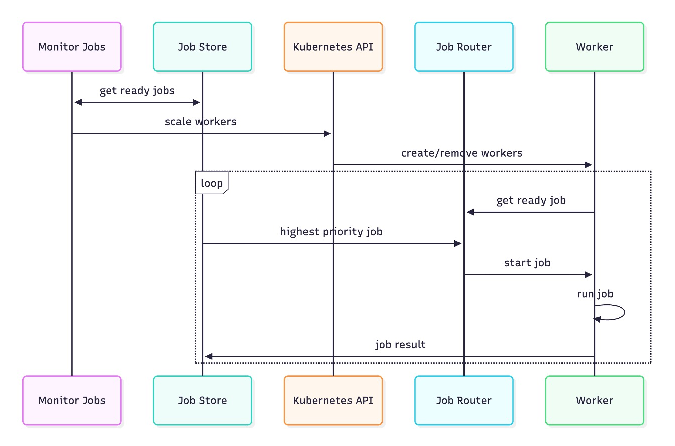
\includegraphics[width=0.92\linewidth]{C401_f2.eps}
\caption{Long-running workers repeatedly obtain jobs from a routing service. Replica counts follow queue depth and resource requirements.}
\label{fig:workers}
\end{figure}

This model amortizes pod scheduling and image initialization over many jobs. Once workers are ready, the interval between jobs falls from the pod-startup timescale of minutes to the routing timescale of less than a second. Memory bins improve node packing by preventing small and large jobs from competing indiscriminately for the same instances. They also provide an explicit control point for limiting expensive or unusually large workloads.

\section{Performance and Operational Experience}

Performance validation has exercised the system at thousands of concurrent jobs. This has resulted in observations of 60 TB of aggregate memory and thousands of vCPUs, while archive ingest has exceeded 1,000 products per minute and reached approximately 3 TB hr$^{-1}$ in high-throughput loads.

Several operational lessons emerged:

\begin{itemize}
  \item \textbf{Autoscaling moves bottlenecks rather than eliminating them.} Once compute provisioning was automated, the limiting components included Kubernetes API activity, database connections, container distribution, and external service quotas.
  
  \item \textbf{Database connections constrain Airflow scaling.} Large numbers of tasks and schedulers create high PostgreSQL connection counts. PgBouncer, connection-pool limits, and database monitoring are therefore required.
  
  \item \textbf{Resource requests affect both cost and throughput.} Inaccurate memory requests reduce node-packing efficiency, while requests that are too small increase the risk of job termination. Resource bins provide predictable behavior but require measurements from representative processing runs.
  
  \item \textbf{Spot capacity should span instance types and zones.} A narrow selection makes bursts harder to provision and increases exposure to interruptions.
  
  \item \textbf{Data transfer costs matter.} Shared file systems, traffic between Availability Zones, and transit gateway traffic can be costly even when compute utilization is efficient.
  
  \item \textbf{Quota monitoring is part of application observability.} EC2, EKS, networking, and downstream-service limits must be monitored alongside task success rates and queue depth. \end{itemize}

\section{Conclusion}

Separating Airflow orchestration from reusable Kubernetes worker pools allows Roman processing to scale elastically while avoiding per-job pod startup overhead. The resulting event-driven architecture has supported operational loads reaching 28,000 vCPUs and provides a reproducible model for other burst-oriented scientific workflows.

\bibliography{C401}

\end{document}
